\section{Introduction}
Semantic Role Labeling (SRL) is a task in Natural Language Processing (NLP) which aims to automatically assign semantic roles to each argument for each predicate in a given input sentence. As for a brief definition, given an input sentence, SRL system will give an output of \textit{"Who did what to whom"} with \textit{what} as the predicate and \textit{who} and \textit{whom} being the argument of the predicate. SRL is an integral part of understanding natural language as it helps machine to retrieve semantic information from the input. In practice, SRL has been widely used as one of the intermediate steps for many NLP tasks, some of which are information extraction [Bastianelli et. al, 2013], machine translation [Liu and Gildea 2010; Lo et al. 2013], question-answering [Dan and Lapata, 2007; Surdeanu et al., 2003, Moschitti et al., 2003].

In the chat bot industry, the bots need to understand semantic information of the user's text in order to generate more personalized response. To illustrate, a scenario is given as follows.

\textit{User: "I just ate fried chicken, bro!"}

\textit{Roles: Agent Predicate Patient"}

By knowing that the user just ate a fried chicken, the bot can thus response with \textit{"That's great! how was the chicken?"}. This way, the user will be more engaged to the conversation with the bot.

As we can see from the example above, it is worth noting that the style of language used on chatting platform is different than those in formal text. In this work, we call this \textit{conversational language}. While formal language has been extensively studied, SRL on conversational language is yet to explore. Since it is informal, the language has some unique characteristics including a wide variety of slangs and abbreviations, short sentences, and disorganized grammars. These characteristics are the challenges an SRL system should tackle in understanding conversational language.

This work explores the SRL on conversational language, including creating a new set of semantic roles and proposing a new architecture, the so-called Context-Aware Bi-Directional Long Short-Term Memory Networks. We utilized word embedding and linguistic components as our main features. The SRL task was mainly evaluated on Indonesian conversational language used on chatting platform. Although this is a pilot task, we obtained a really promising result with F1 score of 74.48\%.

This paper is organized as follows. We first explain the previous works on SRL systems in chapter 2. In chapter 3, the methodology of the research is described, including the features and the model architectures being used. The results and analysis are then explained in chapter 4. Finally, we report our conclusion and potential future works in the last chapter.

\section{Previous Works}
SRL can be seen as either a classification or sequence labeling problem. The earlier research on SRL was conducted with the classification approach, meaning that each argument is being predicted independently from the others. There research focus on how to extract meaningful features out of syntactic parsers, such as path to predicate and constituent type (Gildea et al. 2000, [Gildea et al. 2002]), [Pradhan et al. 2005]. This syntactic information plays a pivotal role in solving SRL problem as it addresses SLR’s long distance dependency [Someone XX]. Thus, traditional SRL system heavily depends on the quality of the parsers. The analysis done by Pradhan et al. (20XX) shows that most errors of the SRL system were caused by the parser's error. In addition, those parsers are costly to build, since it needs linguistic experts to annotate the data. If we want to use our model for another language, we should create the parsers specifically for it, which is another additional work.

In order to minimize the number of hand-crafted features, Collobert et al. (2014) utilize deep learning for solving NLP tasks including Part-of-Speech Tagging, Chunking, and SRL with classification approach. The research aims to prove that one does not need any task-specific feature in order to achieve state-of-the-art performance. The word embedding is used as the main feature across tasks, combined with Convolutional Neural Networks (CNN) architecture to train the model. They achieve promising results for the POS Tagging and Chunking, while for SRL they still need to use features from the parsers to achieve competitive results.

Different from the previous works, Zhou et al. view SRL as a sequence labeling problem in which the arguments are labeled sequentially instead of independently. They proposed an end-to-end learning of SRL using Deep Bi-Directional Long Short-Term Memories (DB-LSTM), with word embedding as the main feature. Their analysis suggests that the DB-LSTM model implicitly extracts the syntactic information over the sentences and thus, syntactic parser is not needed. The research result outperforms the previous state-of-the-art traditional SLR systems as it achieves F1 score of 81,07\%. The research also shows that the performance of the sequence labeling approach using DB-LSTM is better than the classification approach using CNN

While many of the previous works studied SRL on formal language, our research aims to explore SRL on conversational language, which is still under-resourced. We thus introduce a new set of semantic roles for this language type. Furthermore, we propose a new architecture named Context-Aware Bi-LSTM, designed with attention mechanism in order to capture context information of the sentence at a higher level.

\section{Methodology}
In this work, we view the SRL as a sequence labeling problem. Suppose that we have an input of \textit{N} words $w = (w_{1}, w_{2}, ..., w_{n})$, the goal is to find the best sequence of labels $y = (y_{1}, y_{2}, ..., y_{n})$, with $y_{i}$ representing the semantic roles. The probabilities
\begin{equation}
P(y_{i}|w_{i-l}, ..., w_{i+l},y_{i-l}, ..., y_{i+l})
\end{equation}

whereby \textit{l} is a small number. In this chapter, we explain our research methodology including the data annotation, features used, and the proposed model architecture. 

\subsection{Data Annotation}
Since there seems to be no resource available for labeled conversational language data, we annotated our own dataset of Indonesian text chats from Kata.ai’s bots. The data was annotated by three linguists. In this work, we create a new set of semantic roles mainly crafted for informal conversational language. The semantic roles proposed are explained in Table~\ref{tab:semantic_roles}.

\begin{table}
	\caption{Set of Semantic Roles for Conversational Language}
	\label{tab:semantic_roles}
	\begin{tabular}{ll}
		\toprule
		Semantic Roles		&Example\\
		\midrule
		AGENT				& \emph{I} brought you a present\\
		PATIENT				& I brought you \emph{a present}\\
		BENEFICIARY			& I brought \emph{you} a present\\
		GREET 				& Hi \emph{Andy}! I brought you a present\\
		MODAL 				& I \emph{can} eat at home today \\
		LOCATION 			& I can eat at \emph{home} today \\
		TIME 				& I can eat at home \emph{today} \\
		\bottomrule
	\end{tabular}
\end{table}

These semantic roles are inspired by X. The main difference of this set of semantic roles compared to the previous ones is \texttt{GREET}. In conversational language, we often call the name of person we are talking to. This information is useful, for instance, we can derive that "you" refers to "Andy" in "Hi Andy! I brought you a present".

It is worth to note that conversational language has unique characteristics. First, they use slangs and abbreviations. For example, one might use \textit{"u"} instead of \textit{"you"} in \textit{"I brought u a present"}. The grammars are often unstructured and thus, one cannot rely on syntactic parsers to build SRL system for conversational language. The sentences are also filled with interjections such as "haha" and "lol". Lastly, since conversational sentences are really short, averaging around 4-6 words per sentence, it sometimes contains incomplete information. These are the interesting challenges the SRL system should learn and tackle.

\subsection{Features}
We utilized word embedding and POS tag as our main features with neighbouring words as the secondary feature. While most of the SRL research used predicate information as one of the main features, we omit to use it since we seek for an SRL system which finds the predicate from scratch alongside with other semantic roles.

We train the word embedding model with our chat corpus using Word2Vec’s Skipgram architecture (Mikolov et al., 2013). The corpus contains X tokens. All the words were lowercased before being fed into the model. The trained word embedding model contains vocabulary size of X. The context window and word dimension parameters used are 5 and 32, respectively.

We use the gold-standard POS tag on our data as the second feature. Even though deep learning model aims to pr We argue that POS tag is still important for building a robust model. Nonetheless, building POS tags model is way easier than building syntactic or dependency parsers.

As an additional feature, we also experiment with neighbouring words features with context window of 3. Suppose that we are in t timestep, the neighbouring words are the word embeddings of timestep t-1 and t+1. This feature can be useful for capturing the context of the word by looking at the words around it.

\subsection{Context-Aware B-LSTM}
Recurrent Neural Networks (RNN) has a nature advantage for solving sequence labeling problem (Zhou et al., 2015). In this work, we propose a new RNN architecture named Context-Aware Bi-Directional Long Short-Term Memory Networks (CAB-LSTM). The rationale is to add a dense yet useful information containing a sentence context to every time step in order to help the machine decide semantic roles better. With this in mind, we design an attention mechanism on top of the recurrent networks layers, as illustrated in Figure~\ref{fig:cabilstm} 

The attention mechanism firstly collects the context information by multiplying trainable weights with all the vectors from every time step of the last LSTM output. We sum each element for each weighted vectors to reduce the dimension. The results are then fed into a hidden softmax layer which outputs distributed weights with a total of 1. The original output vectors of the last LSTM output are multiplied by these distributed weights respectively. We then sum all the multiplication results as the final context information. The original LSTM outputs are concatenated with this context information before going to the last softmax layer to predict the semantic roles.

The formula of this attention mechanism is described as follows.
(W21, W22, …, W2t) = softmax(tanh(W1. V1 + W2. V2 + … + Wt Vt))
Z = W21. V1 + W22. V2 + … + W2t. Vt

With V1, V2, …, Vt as the last LSTM output vectors, W1, W2, Wt as the trainable weights, W21, W22, W2t as the final weight of every time step. The context information is denoted as Z. Z is concatenated with all the vectors V1, V2, .., Vt as the additional information to predict the semantic roles in the last softmax output layer.

\begin{figure}
	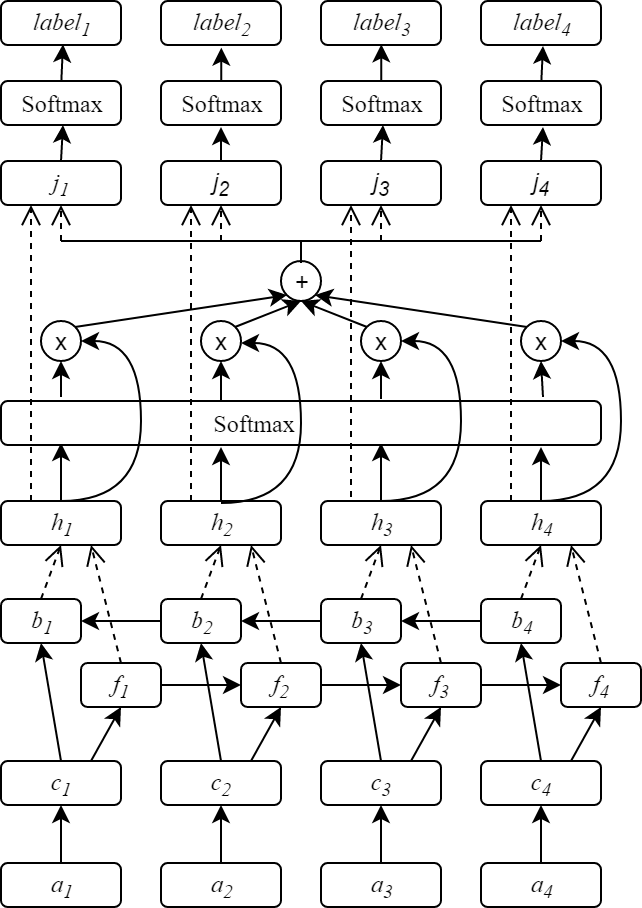
\includegraphics[width=3in]{cabilstm}
	\caption{An architecture of Context-Aware Bi-Directional Long Short Term Memories.}
	\label{fig:cabilstm}
\end{figure}

\section{Experiments}
In this chapter, we focus on presenting our experiment results and the analysis accordingly. There are two set of scenarios. The first scenario set aims to find the best combination of features. This scenario consists of four combinations as follows:

\begin{enumerate}
	\item Word Embedding (WE)
	\item Word Embedding + POS Tag (WE + POS)
	\item Word Embedding + Word Embedding of Neighbors (WE + WE-N)
	\item Word Embedding + POS Tag + Word Embedding of Neighbors (WE + POS + WE-N)
\end{enumerate}

The second scenario set evaluates two different architectures, which are the original BI-LSTM and CABI-LSTM. Underlying both architectures is a Convolutional Neural Network (CNN) layer, in order to catch more information surrounding each time step. This second scenario also aims to see the effect of hyper-parameter tuning for the CABI-LSTM.

\subsection{Evaluation Metrics}
As for evaluation, we use precision, recall and F1 metrics for all scenarios. The results are evaluated with partial match approach (XX et al., 20XX).

\subsection{Feature Combination Scenario}
Table~\ref{tab:feature_scenario} shows the scenario results of four feature combinations. The highest result is achieved with combination of WE + POS, followed by WE + WE-N + POS, WE, and WE + WE-N, with F1 scores of 72.29\%, 72.22\%, 62.00\%, and 61.92\% respectively. From these results, we can see the big impact POS Tag contributes for the performance. Using POS Tag enhances the result up to 10.29\%, when we compare WE + POS and WE combinations. The explanation would be the fact that POS Tag contains meaningful information such as Noun and Adjective which describes the word, it thus supports the word embedding feature.

Surprisingly, when we combine the neighboring words of the argument as in WE + WE-N, the result slightly decreases by 0.08\%, compared to only using WE feature. This is also the case when we compare WE + WE-N with WE + WE-N + POS scenarios, which decreases by 0.07\% when we used neighboring words. It tells us that neighbouring words do not improve the performance at all. We suggest that this is because the CNN layer already extracts these information implicitly, by capturing surrounding information and compressed it into one vector. Hence, we do not need an explicit neighboring words as part of our features. 

\begin{table}
	\caption{Results of Feature Combination Scenario}
	\label{tab:feature_scenario}
	\begin{tabular}{llll}
		\toprule
		Features		&Precision	&Recall		&F1			\\
		\midrule
		WE				&	64.68\%				&	60.25\%				&	62.00\%	\\
		WE + POS		&	74.24\%				&	\textbf{71.26\%}	&	\textbf{72.29\%}	\\
		WE + WE-N		&	64.17\%				&	60.29\%				&	61.92\%	\\
		WE + POS + WE-N	&	\textbf{74.51\%}	&	70.69\%				&	72.23\%	\\
		\bottomrule
	\end{tabular}
\end{table}

Since WE + POS outputs the best result in terms of F1 score in this scenario set, we will use it for the next set of scenarios.

\subsection{Model Architecture Scenario}
The experiment results of the second scenario set are presented in Table~\ref{tab:architecture_scenario}. The results show that the CABI-LSTM architecture outperforms the original BI-LSTM architecture. The highest F1 is achieved by CABI-LSTM 256. The most drastic improvement here is the precision. The precision started to increase with dimension 128 by 2.00\%, compared to the original BI-LSTM (76.25\% vs 74.24\%). When we added more dimension to the weight, 256, the precision increases by 3.10\%, compared to the original one. When the system is more context-aware to predict every time step, it becomes more careful when predicting a label. Hence, the number of precision increases, since when it predicts, it predicts carefully. 

The best recall is on the weight 128with 73.52\%. It increases by 2.2\%.

\begin{table}
	\caption{Results of Model Architecture Scenario}
	\label{tab:architecure_scenario}
	\begin{tabular}{llll}
		\toprule
		Name			&Precision					&Recall		&F1			\\
		\midrule
		BI-LSTM				&	74.24\%				&	71.26\%				&	72.29\%	\\
		CABI-LSTM-64		&	73.37\%				&	73.25\%				&	73.05\%	\\
		CABI-LSTM-128		&	76.25\%				&	73.52\%				&	74.05\%	\\
		CABI-LSTM-256		&	\textbf{77.03\%}	&	\textbf{73.55\%}	&	\textbf{74.78\%}\\
		\bottomrule
	\end{tabular}
\end{table}


\section{Conclusions}

%\end{document}  % This is where a 'short' article might terminate


\begin{acks}
  The authors would like to thank Dr. Yuhua Li for providing the
  matlab code of  the \textit{BEPS} method. 

  The authors would also like to thank the anonymous referees for
  their valuable comments and helpful suggestions. The work is
  supported by the \grantsponsor{GS501100001809}{National Natural
    Science Foundation of
    China}{http://dx.doi.org/10.13039/501100001809} under Grant
  No.:~\grantnum{GS501100001809}{61273304}
  and~\grantnum[http://www.nnsf.cn/youngscientsts]{GS501100001809}{Young
    Scientsts' Support Program}.

\end{acks}
